\def\numOfLex{17}
\def\numOfFun{8}
\def\gray#1{{\color{gray}\char`<#1\char`>}}
\newcommand{\tts}[1]{{\tt #1}}
% \newcommand{\quality}[1]{${\tt AP_{#1}}$}
% \newcommand{\kind}[1]{${\tt CN_{#1}}$}
% \newcommand{\very}[1]{${\tt Very_{#1}}$}
% \newcommand{\comment}{${\tt S}$}
% \newcommand{\modFun}[2]{${\tt Mod_{#1\times#2}}$}
% \newcommand{\predFun}[3]{${\tt Pred_{#1\times#2\times#3}}$}
% \newcommand{\itemSpa}[2]{${\tt NP_{#1\times#2}}$}
% \newcommand{\itemEng}[1]{${\tt NP_{#1}}$}

\chapter{Test Case Generation for Grammatical Framework}
\label{chapterGFtest}

\epigraph{\it Fixpoint computation is the new SAT I'm afraid.}{Koen
  Claessen, 2018}

\noindent What is the \emph{essence} of a language? When formalising
and implementing a natural language grammar, which example sentences
do we need to check in order to convince ourselves that the grammar is
correct? 
% Previously, we have enforced an internal logic to the grammar rules,
% without needing any interaction with the external world. We have taken
% for granted that the humans who write the rules know what they are
% doing; and even if this assumption is false, there are already methods
% that test whether a given rule takes effect in a corpus.

Imagine we are formalising a grammar for English, and in particular we
are working on the reflexive construct. In order to check correctness
for the 3rd person singular, we need to test for three different
subjects, because the object has to agree with the subject: ``he sees
himself'', ``she sees herself'' and ``it sees itself''. Without seeing
all three examples (along with the rest of the pronouns), we cannot be certain that the reflexive
construction is implemented correctly. In contrast, the general
pattern of a transitive verb with a non-reflexive object is enough to
test with only one third person subject: \emph{he, she, it}, or any
singular noun or proper name. The agreement only shows in the verb
form, thus including both ``she sees a dog'' and ``John sees a dog''
in the test suite is redundant.  

Now, what is minimal and representative is highly language-dependent. 
For instance, Basque transitive verbs agree with both subject and
object, thus we need 6 $\times$ 6 examples just to cover all verb
forms. In this chapter, we are not interested in the morphology per se---there are
easier methods to test for that---but the correctness of the syntactic
function: does the function pick the correct verb form for the correct
combination of subject and object? For that purpose, it is enough to
test the syntactic construction ``transitive verb phrase'' with just a
single transitive verb.

We present a method that, given a grammar (that in general encompasses
an infinite set of sentences), generates a finite set of sentences
that can be used as test cases for the correctness of the grammar. Our
concrete implementation is for a particular grammar formalism, namely
parallel multiple context-free grammars (\pmcfg) \cite{seki91pmcfg},
which is the core formalism used by the Grammatical Framework (\gf)
\cite{ranta2004gf}. However, the general method works for any
formalism that is at most as expressive as \pmcfg{}, including
context-free grammars, formalisms such as Tree-Adjoining Grammar
(\tagGrammar) \cite{joshi1975tag}, and several variants of Categorial
Grammar \cite{deGroote2004,steedman1988ccg}.

The following sections assume knowledge of \gf{} and \pmcfg{}
formalisms; we direct the reader to Section~\ref{sec:gf-intro} for a
general \gf{} introduction, and \ref{sec:PMCFG} especially for
translation of a \gf{} grammar into \pmcfg{}.


\section{Related work}

Traditionally, \gf{} grammars are tested by the grammarians
themselves, much in the way described in the introduction of this
article. An example human-written treebank can be found in
\citet[p.~136--142]{khegai2006phd}.  For testing the coverage of the
grammars, grammarians have used treebanks such as the UD treebank
\cite{nivre2016ud} and Penn treebank \cite{marcus1993penntreebank},
and for testing morphology, various open-source resources have been
used, such as morphological lexica from the Apertium project
\cite{forcada2011apertium}.

As an example of other grammar formalisms,
\citet[pp.~212--213]{butt1999lfg} describe common methods of testing
the \lfg{} formalism: similarly to \gf, they use a combination of
human-written test suites meant to cover particular phenomena, and
external larger corpora to test the coverage. As a difference from
\gf{} testing tradition, their human-written test suites include also
ungrammatical sentences: those that the grammar should \emph{not} be
able to parse. However, their tests are only meant for monolingual
grammars, whereas \gf{} tests are for multilingual grammars, so they
are stored as trees. In other words, \gf{} tests only what the grammar
outputs, not what it parses.

Other related work in computational linguistics includes error mining
for parsing grammars, such as \citet{gardent2012errormining}. The
setup includes triples of dependency tree, generated sentence and the
gold standard sentence. For every triple where the generated sentence
and the gold standard sentence are different, their algorithm finds
the smallest subtrees that cause the problems. Gardent's algorithm
fills a slightly different need than ours: it relies on the correct
linearisation so be known, which we don't. Instead, we want to
generate trees whose linearisations are then read by humans. On the
other hand, Gardent's method would prove very useful once an error is
found---it can be tricky to determine which function exactly caused
the error.  Further away from our approach, \citet{vanNoord2004} works
on parsing grammars rather than generation, with the goal of detecting
strings that cause parsing errors.

However, our biggest source of inspiration is automatic test case
generation for general software, such as
\citet{celentano1980compiler,Geist1996,QuickCheck}. Software testing and
grammar testing both deal with notions of coverage and compactness,
and deriving test cases from a formal specification. Sometimes even
software tests are generated with human oracles in mind, such as in 
\citet{Matinnejad2016automated_testsuite_simulink}.


\section{Grammar}


\begin{figure}[h]
  \centering
\begin{Shaded}
\begin{Highlighting}[]
\NormalTok{abstract }\DataTypeTok{NounPhrases} \FunctionTok{=} \NormalTok{\{}
  \NormalTok{flags startcat }\FunctionTok{=} \DataTypeTok{NP} \NormalTok{;}
  \NormalTok{cat}
    \DataTypeTok{S} \NormalTok{; }\DataTypeTok{NP} \NormalTok{; }\DataTypeTok{Adv} \NormalTok{;                       }\CommentTok{-- Non-terminal categories}
    \DataTypeTok{CN} \NormalTok{; }\DataTypeTok{Det} \NormalTok{; }\DataTypeTok{Adj} \NormalTok{; }\DataTypeTok{Prep} \NormalTok{;              }\CommentTok{-- Terminal (lexical) categories}
  \NormalTok{fun}
    \DataTypeTok{UttNP}   \FunctionTok{:} \DataTypeTok{NP} \OtherTok{->} \DataTypeTok{S} \NormalTok{;                  }\CommentTok{-- Single NP as an utterance}
    \DataTypeTok{PredAdj} \FunctionTok{:} \DataTypeTok{NP} \OtherTok{->} \DataTypeTok{Adj} \OtherTok{->} \DataTypeTok{S} \NormalTok{;           }\CommentTok{-- e.g. "this house is blue"}
    \DataTypeTok{PredAdv} \FunctionTok{:} \DataTypeTok{NP} \OtherTok{->} \DataTypeTok{Adv} \OtherTok{->} \DataTypeTok{S} \NormalTok{;           }\CommentTok{-- e.g. "this house is on a hill"}
    \DataTypeTok{DetNP} \FunctionTok{:} \DataTypeTok{Det} \OtherTok{->} \DataTypeTok{NP} \NormalTok{;                  }\CommentTok{-- e.g. "this"; "yours"}
    \DataTypeTok{DetCN} \FunctionTok{:} \DataTypeTok{Det} \OtherTok{->} \DataTypeTok{CN} \OtherTok{->} \DataTypeTok{NP} \NormalTok{;            }\CommentTok{-- e.g. "this house"}
    \DataTypeTok{PrepNP} \FunctionTok{:} \DataTypeTok{Prep} \OtherTok{->} \DataTypeTok{NP} \OtherTok{->} \DataTypeTok{Adv} \NormalTok{;         }\CommentTok{-- e.g. "without the house"}
    \DataTypeTok{AdjCN} \FunctionTok{:} \DataTypeTok{Adj} \OtherTok{->} \DataTypeTok{CN} \OtherTok{->} \DataTypeTok{CN} \NormalTok{;            }\CommentTok{-- e.g. "small house"}
    \DataTypeTok{AdvCN} \FunctionTok{:} \DataTypeTok{Adv} \OtherTok{->} \DataTypeTok{CN} \OtherTok{->} \DataTypeTok{CN} \NormalTok{;            }\CommentTok{-- e.g. "house on a hill"}

    \NormalTok{a, the, this, these, your }\FunctionTok{:} \DataTypeTok{Det} \NormalTok{;}
    \NormalTok{good, small, blue, tired, ready }\FunctionTok{:} \DataTypeTok{Adj} \NormalTok{;}
    \NormalTok{house, hill }\FunctionTok{:} \DataTypeTok{CN} \NormalTok{;}
    \NormalTok{in, next_to, on, with, without }\FunctionTok{:} \DataTypeTok{Prep} \NormalTok{; }
\NormalTok{\}}
\end{Highlighting}
\end{Shaded}
  \caption{\gf{} grammar for noun phrases}
\label{fig:exampleGrammar}
\end{figure}

Figure~\ref{fig:exampleGrammar} shows a small example of a \gf{}
abstract grammar. The grammar generates noun phrases for a lexicon of
\numOfLex{} words (\emph{a, the, \dots, without}) in four lexical
categories, and \numOfFun{} functions to construct phrases. \t{CN} stands
for common noun, and it can be modified by arbitrarily many adjectives
(\t{Adj}), e.g. \emph{small blue house} is an English linearisation of
the abstract syntax tree \t{AdjCN small (AdjCN blue house)}. A \t{CN}
is quantified into a noun phrase (\t{NP}) by adding a determiner
(\t{Det}), e.g. \emph{the small house} corresponds to tree \t{DetCN
  the (AdjCN small house)}. Alternatively, a \t{Det} can also become
an independent noun phrase (as in, \emph{(I like) this} instead of
\emph{(I like) this house}) using the constructor \t{DetNP}. Finally,
we can form an adverb (\t{Adv}) by combining a preposition (\t{Prep})
with an \t{NP}, and those adverbs can modify yet another \t{CN}.  We
refer to this grammar throughout the chapter.

\subsection{Examples to test}
\label{gf-testing-examples}

As examples that help illustrate different testing needs for different
languages, let us take four language-specific phenomena in the scope
of our small grammar: preposition contraction in Dutch, adjective
agreement in Estonian, adjective placement and agreement in Spanish
and determiner placement in Basque. Concrete syntaxes for all four
languages are found in
\url{https://github.com/inariksit/GF-testing/tree/master/data/grammars};
however, the chapter can be read without understanding the details of
the concrete syntaxes.

\paragraph{Preposition contraction in Dutch} In Dutch, some prepositions should
merge with a single determiner or pronoun, e.g. \emph{met~dit} `with
this' becomes \emph{hiermee} `herewith', but stay independent when the
determiner quantifies a noun, e.g. \emph{met~dit~huis} `with this house'. 
Other prepositions, such as \emph{zonder} `without', do not
contract with any determiners: \emph{zonder~dit} `without this' and
\emph{zonder~dit~huis} `without this house'.
When testing \t{PrepNP}, we would like to see one preposition that
contracts and one that does not, as well as one \t{NP} that is a
single determiner, and one that comes from a noun. Since the result of
\t{PrepNP} is an adverb, which does not inflect any further, we are
happy with just finding the right arguments to \t{PrepNP}, no need for contexts.
In order to catch a bug in the function, or confirm there is none, we
need the following 4 trees: 

\[
\t{PrepNP}\; \{ \stackanchor{\tt with}{\tt without} \} 
           \{ \stackanchor{\tt DetNP this}{\tt DetCN this house} \}. 
\]

\paragraph{Adjective agreement in Estonian} In Estonian,
most adjectives agree with nouns in case and number in an attributive
position. However, participles are invariable (singular nominative) as 
attributes but inflect regularly in a predicative position, and a set
of invariable adjectives do not inflect in any position. Furthermore,
in 4 of the 14 grammatical cases, even the regular adjectives only
agree with the noun in number, but the case is always genitive.
Table~\ref{estonian} shows the different behaviours in attributive
position, with \emph{sinine} `blue' as an example of a regular
adjective, and \emph{valmis} `ready' as an invariable.

\begin{table}[h]
\small
\begin{tabular}{ll | ll | ll}

\multicolumn{2}{c|}{\bf Regular} & \multicolumn{2}{c|}{\bf Genitive
                                   agreement} & \multicolumn{2}{c}{\bf
                                                Invariable} \\ \hline
 sinises & majas &  sinise & majaga &  valmis & majas \\
blue-{\sc sg.ine} & house-{\sc sg.ine} & blue-{\sc sg.gen} & house-{\sc sg.com} &  ready.{\sc sg.nom} & house-{\sc sg.ine} \\
\multicolumn{2}{l|}{`in a blue house'} & \multicolumn{2}{l|}{`with a blue house'} & \multicolumn{2}{l}{`in a finished house'} \\
 & & & & & \\
sinistes & majades & siniste & majadega & valmis & majades \\
blue-{\sc pl.ine} & house-{\sc pl.ine} & blue-{\sc pl.gen} & house-{\sc pl.com} & ready.{\sc sg.nom} & house-{\sc pl.ine} \\
\multicolumn{2}{l|}{`in blue houses'} & \multicolumn{2}{l|}{`with blue
                                         houses'} &
                                                     \multicolumn{2}{l}{`in finished houses'}

\end{tabular}
\caption{Estonian adjective agreement}
\label{estonian}
\end{table}

% \begin{table}[h]
% \begin{tabular}{cllcll}
% (1) & suur-e        &  auto-ga       & (2) & suur-te  & auto-de-ga \\ 
%     & big-{\sc gen} &  car-{\sc com} &  & big-{\sc pl.gen} & car-{\sc pl-com} \\
%     & \multicolumn{2}{l}{`with (the) big cars'} 
%                                      &  & \multicolumn{2}{l}{`with (the) big cars'} \\
% \end{tabular}
% \end{table}

%\stackanchor{ \emph{suur-e} \emph{auto-ga}}{\small
%\emph{big}-\textsc{gen} \emph{car}-\textsc{com}} 

%\emph{suur-e} \emph{auto-ga}  \emph{big}-{\sc sg.gen} \emph{car}-\textsc{com} `with a big car'. 
% \noindent Thus in order to test adjectives as attributes, we need an
% example for one of the 10 ``usual'' cases and one of the 4 ``unusual''
% cases, one of each type of adjective, and one of each number. 
\noindent Since we are interested in adjectives, choosing \t{AdjCN} as
the base sounds reasonable---but that only creates an inflection
table, so we must think of a context too. Just like in English, number
comes from the determiner, so we need to wrap the \t{CN} in a \t{DetCN}
with two determiners of different number, for instance \t{this} and
\t{these}. But we still need an example for one of the 10 cases with
normal agreement, such as inessive (in something), and one of the 4
cases with restricted agreement, such as comitative (with something).
These cases correspond to the English prepositions \emph{in} and \emph{with},
so in this abstract syntax we can use \t{PrepNP} with the arguments
\t{in} and \t{with}. This is another showcase of the abstraction level
of \gf{}: in the English concrete syntax, \t{Prep} contains a string
such as `in' or `with', and \t{PrepNP} concatenates the string from its
\t{Prep} argument into the resulting adverb, but in Estonian, \t{Prep}
contains a case, and \t{PrepNP} chooses that case from its \t{NP} argument.
The following set of 8 trees creates all the relevant
distinctions:
% \footnote{If the grammar covered predicative
% constructions, we would need a participle in the test set. As an
% attribute, we do not need both participles and invariables,
% because they behave identically, but as a predicative, regular and
% participle adjectives behave the same, and differently from
% invariable.}: 
\[
 \t{PrepNP} \; \{ \stackanchor{\tt in}{\tt with} \} \;
             \t{(DetCN} \; \{ \stackanchor{\tt this}{\tt these} \}
             \; 
             \t{AdjCN} \; \{\stackanchor{\tt blue}{\tt ready} \} 
             \; \t{house)}.
\]
% If we wanted to test \emph{adjectives} exhaustively, we would need one more context, where
% the adjective is in the predicative position: e.g. `the house is \verb|_|'.
% Furthermore, we need to add a participle to the test cases.
% As an attribute, we do not need both participles and invariables,
% because they behave identically, but as a predicative, regular and
% participle adjectives behave the same, and differently from
% invariable. If we want to test specifically adjectives and not
% \t{PrepNP}, we would prefer to see all types in all positions:
%  \t{PrepNP} \{ \stackanchor{\tt in}{\tt with} \}
%              {\tt (DetCN} \{ \stackanchor{\tt this}{\tt these} \} 
%              {\tt AdjCN}  \{\stackanchor{\tt blue}{\stackanchor{\tt
%                  ready}{\tt tired}} \} 
%              {\tt house)}.


\paragraph{Adjective placement and agreement in Spanish}
Spanish adjectives agree in number and gender with the noun, in both
attributive and predicative position. In attributive position, most
adjectives (e.g. \t{small}) come after its head, but some adjectives
(e.g. \t{good}) are placed before the head. 
In order to test \t{AdjCN}, with regards to both adjective placement
and agreement, we need the following 8 trees: 
\[
\t{DetCN} \; \{ \stackanchor{\tt this}{\tt these} \} \;
 \t{(AdjCN} \; \{ \stackanchor{\tt good}{\tt small} \} 
           \{ \stackanchor{\tt house}{\tt hill} \}\t{)}.

\paragraph{Determiner placement in Basque} In Basque, there are three
different ways to place a determiner into a noun phrase. When a number
(other than 1) or a possessive pronoun acts as a determiner in a
complex noun phrase, it is placed between ``heavy'' modifiers, such as
adverbials or relative clauses, and the rest of the noun phrase. 
Demonstrative pronouns, such as \emph{this}, are placed after
all modifiers as an independent word. Number 1, which functions as an
indefinite article, acts like demonstratives, but the definite article
is a suffix. If there is a ``light'' modifier, such as an adjective,
the definite article attaches to the modifier; otherwise it attaches
to the noun. 
In order to test the implementation of this phenomenon,
we need the following 12 trees: 

\[
\t{DetCN} \; \{
\stackanchor{\stackanchor{}{\tts{the}}}{\stackanchor{\tts{this}}{\tts{your}}}
\} \; \{ \stackanchor{\tt AdvCN on (DetCN the hill)}{$\varnothing$} \} \;
\{ \stackanchor{\tt AdjCN small}{$\varnothing$} \} \; \t{house}.
\]
\section{Using the tool}

Here is a typical use for the tool. Let us take the noun phrase
grammar for Dutch, and pick a single function, say \t{AdvCN}. We
generate test cases, which include the following trees:
\begin{itemize}
\item[] \t{AdvCN (PrepNP next\_to (DetNP your)) hill} \\
`hill next to yours'
\item[] \t{AdvCN (PrepNP next\_to (DetNP your)) house} \\ `house next
to yours'
\end{itemize}
In Dutch, the words \emph{hill} and \emph{house} have different
genders, and the word \emph{yours} has to agree in gender with the
antecedent: \emph{(de) heuvel naast de jouwe} and \emph{(het) huis
  naast het jouwe}. Say that the test cases reveal a bug, where
\t{DetNP your} picks a gender too soon---always neuter, ``het jouwe'',
instead of leaving it open in an inflection table. To fix the bug, we
add gender as a parameter to the \t{Adv} type, and have \t{AdvCN}
choose the correct form based on the gender of the \t{CN}.

After implementing the fix, we run a second test case generation: this
time, not meant for human eyes, but just to compare the old and new
versions of the grammar. We want to make sure that our changes to
\t{Adv}, \t{AdvCN} and \t{DetNP} have not caused new bugs in other
categories and functions. The simplest strategy is to generate test
cases for \emph{all} functions in both grammars, and only show those
outputs that differ between the grammars. After our changes, we get
the following differences:
\newpage
\begin{itemize}
\item[] \t{DetCN the (AdvCN (PrepNP next\_to (DetNP your)) hill)}
  \begin{itemize}
   \item \emph{\sout{de heuvel naast {\bf  het} jouwe}}
   \item[+] \emph{de heuvel naast {\bf  de} jouwe}
  \end{itemize}
\item[] \t{DetCN the (AdvCN (PrepNP without (DetNP this)) hill)}
  \begin{itemize}
   \item \emph{\sout{de heuvel zonder {\bf  dit}}}
   \item[+] \emph{de heuvel zonder {\bf  deze}}
  \end{itemize}
\end{itemize}

We notice a side effect that we may not have thought of: the
gender is retained in all adverbs made of NPs made of determiners, so
now it has become impossible to say ``the hill next to \emph{that}'',
where \emph{that} is referring to a house. So we do another round of
modifications, compute the difference (to the original grammar or to
the intermediate), and see if something else has changed.

\paragraph{Additional analyses}
Aside from concrete language-dependent phenomena, there are more
general questions a grammar writer may ask. For instance, say that our
concrete type for \t{CN} in some language is an inflection table from
case to string, we would like to know if (a) a given string field is
unreachable from the start category; (b) any two fields always contain
the same string; or (c) some fields are always the empty string.  In
addition, a whole argument may be erased by some function: say that
\t{AdjCN~:~Adj~$\rightarrow$~CN~$\rightarrow$~CN} never adds the
adjective to the new \t{CN}, in which case \t{AdjCN blue house} and
\t{house} are linearised identically. Instead of testing every single
function and finding out by accident, we can test the whole grammar to
find out if there are any functions in the grammar that behave like
this. %\todo{Should these be explained too later?}


%  We have seen that, in order to test
% whether or not we have implemented a linguistic phenomenon correctly,
% we take a single function as a base, and describe all combinations of
% arguments that are needed to test the function. If the result of the
% function is an inflection table rather than a fully specified result,
% then we need several \emph{contexts} to squeeze out all the different
% forms. For example, a \t{CN} in English is open for number---\t{house}
% is really a table \{\t{Sg~=>}~\emph{``house''}~\t{;~Pl~=>}
% \emph{``houses''}\}, and applying a determiner chooses the right form:
% \t{DetCN~this~house} linearises to \emph{this house} and \t{DetCN
%   these house} linearises to \emph{these houses}. 

% \label{sec:wishlist_comments}
% The example grammar, with only \numOfLex{}-word lexicon and \numOfFun{} syntactic functions,
% generates over 10,000 %17,574
% trees\footnote{e.g. {\tt DetCN the (AdvCN (PrepNP on
% (DetCN a (AdjCN small hill)) (AdjCN blue house))} `the blue house on a
% small hill'}  up to depth 5. 
% However, as we have seen in the examples above, we can test complex
% morphosyntactic phenomena with just a set of 4, 8 or 12 trees,
% depending on the complexity of the language. 

% As mentioned previously, the base of a test case is one syntactic
% function, but often the same sentence ends up showcasing several
% functions. In the Estonian example, we start from \t{AdjCN} 
% and end up in a context formed by \t{PrepNP}---in fact, these 8 trees
% cover all tests we would've needed for \t{PrepNP} itself. Thus,
% it is possible to shrink the test cases effectively, if one wants to
% test the whole grammar at one go.

% Of course, such a test set will not catch e.g. individual
% misspellings, or more systematic bugs in the morphological
% paradigms. But there are easier methods to test for such bugs---our 
% goal is to test the more abstract, syntactic phenomena with as few
% trees as possible.  


\section{Generating the test suite}
\label{sec:testing}

In this section, we explain how the test suites are built.
Earlier in Section~\ref{sec:PMCFG}, we saw how a single abstract category
compiles into multiple concrete categories $N^C$, depending on the
combinations of parameters. Instead of dealing with parameters
directly, we now have a set of new \emph{types}, which is helpful for
generating test cases.

We use one syntactic function as the base for one set of test
cases. For lexical categories, it also makes sense to test the whole
category, i.e. generate all trees that show that \t{AP} is defined and
handled correctly in the functions. However, we only explain in detail
the method with one syntactic function as a base.

We assume that all test cases are trees with the same start
(top-level) category, such as \t{S} in our example grammar. The
requirement is that the start category is linearised as one string only. 

%\paragraph{Notation}


\subsection{Enumerate functions} As we explained before, each
syntactic function in the abstract syntax turns into multiple
versions, one for each combination of parameters of its arguments.  In
the notation by \citet{angelov2010phd}, presented in
Section~\ref{sec:PMCFG}, these concrete functions are the set $F^C$.

In order to construct trees that use the concrete syntactic function
$f$, we need to supply the function with \emph{arguments}, as well as
put the resulting tree into a \emph{context} that produces a tree in
the correct start category.  In the best case, each $f$ produces only
one tree, but as we will explain in the following section, sometimes
we need more than one tree for a single concrete function; this
happens if there are no arguments with unique string fields.



\subsection{Enumerate arguments} 
\label{enumerate-arguments}
Some syntactic functions are simply a single lexical item (for example
the word \emph{good}); in this case just the tree \t{good} is our
answer.  If we choose a function with arguments, such as \t{PrepNP},
then we have to supply it with argument trees. Each argument needs to
be a tree belonging to the right category (in the example, \t{Prep}
and \t{NP}, respectively).

When we test a function, we want to see whether or not it uses the
right information from its arguments, in the right way. The
information that a syntactic function uses is any of the strings that
come from linearising its arguments. In order to be able to see which
string in the result comes from which field from which argument, we
want to generate test cases that only contain unique strings.  For
example, the English pronoun {\em you} is a worse test case than {\em
  they}, because all forms are not unique: {\em you} is both
nominative and accusative ({\em you} sleep vs. I saw {\em you}),
whereas {\em they} has a different form for both ({\em they} sleep
vs. I saw {\em them}).


\paragraph{Subsumption} For our testing purposes, any other pronoun
with all unique forms \emph{subsumes} the pronoun {\em you}: if we can
construct a test with \{{\em they},{\em them},{\em their}\}, we don't
need the inferior \{{\em you},{\em you},{\em your}\} in addition. In
general, we would like to find just one combination of arguments where
all strings in the linearisations are different. However, it is not
always possible to do this, which is why we in general aim to generate
a set of combinations of arguments, where for each pair of strings
from the arguments, there is always one test case where those strings
are different. If all pronouns in English were non-unique, we could
still get the effect by using both \{{\em you},{\em you},{\em your}\}
and \{{\em she},{\em her},{\em her}\}, because their ambiguity
manifests in different forms\footnote{The majority of all functions in all tested languages need 1 or
2 argument trees, and there are only a handful of cases that need more
than 3. The highest number we encountered was 8 trees, for a single
function in the Basque resource grammar.}.
% for the Basque
% function which handles conjunctions of the category \t{DAP}
% (determiner with an adjective, e.g. ``three small'').

We define the function $\textsf{subsumes}$ for a given function $f$
and two candidate lists of argument trees. It is important to include
the function $f$ and not just its arguments, because any \gf{}
function may introduce new strings to the linearisation. If $f$
introduces some string $s$, then any argument that contains $s$ is
worse than an otherwise identical argument without $s$.

In addition to \citet{angelov2010phd}'s definition, we use the notion of
$\textsf{Tree}$ as a generic type for any application of some
$f \in F^C$ to all of its arguments $[A_1, \dots, A_{a(f)}]$.  Thus, a
single $f \in F^C$ is also a $\textsf{Tree}$, if $a(f) = 0$. For an
$f$ with $a(f) > 0$, we need to apply $f$ to $a(f)$ argument
$\textsf{Tree}$s.


\begin{EmptyItem}
\begin{array}{p{0.25cm} p{0.2cm} l}
% \multicolumn{3}{l}{\textsf{subsumesString : [String]} \rightarrow
%   \textsf{[String]}\rightarrow \textsf{Bool}} \\
% \multicolumn{3}{l}{\textsf{subsumesString xs ys} =} \\
%  & \multicolumn{2}{l}{\forall i,j : \textbf{ if } \textsf{xs } ! \, i =
%    \textsf{xs } ! \, j,
%    \textbf{ then also } \textsf{ys } ! \, i = \textsf{ys } ! \, j.} \\
% \\
\multicolumn{3}{l}{\textsf{subsumes : }F^C \rightarrow \textsf{[Tree]} \rightarrow \textsf{[Tree]} \rightarrow \textsf{Bool}} \\
\multicolumn{3}{l}{\textsf{subsumes } f \textsf{ xtrees ytrees} =} \\
 & \textbf{let} & \textsf{xlins} = \textbf{strings of}
    \textsf{ xtrees}\text{ ++ }\textbf{strings that } f \textbf{
                  introduces} \\
 &              & \textsf{ylins} = \textbf{strings of}
    \textsf{ ytrees}\text{ ++ }\textbf{strings that } f \textbf{
                  introduces} \\
 & \textbf{in}  & \forall i,j : \textbf{ if } \textsf{xlins } ! \, i =
   \textsf{xlins } ! \, j,
   \textbf{ then also } \textsf{ylins } ! \, i = \textsf{ylins } ! \,
                  j. \\
%\textsf{subsumesString xlins ylins} \\
\end{array}
\end{EmptyItem}

\paragraph{Argument generation and filtering}
For a given $f \in F^C$, we generate all lists of argument trees
$[A_1, \dots, A_{a(f)}]$.  We keep the ones we need to test $f$, such
that all forms have a unique string, using the previously defined
function $\textsf{subsumes}$.

The function $\textsf{generateAllTrees}$ is implemented using the
\feat{} library \cite{feat}, and generates lazily all vectors of
argument trees for the given concrete categories, starting from
smallest size.  The size of a tree is defined as the number of
constructors; thus \t{DetNP~this} is generated before \t{DetCN this
  house}. This ensures that we find the most minimal and the most
unique examples.


\begin{EmptyItem}
\begin{array}{p{0.25cm} p{0.2cm} l}
\multicolumn{3}{l}{\textsf{generateAllTrees :: [}N^C\textsf{]} \rightarrow
  \textsf{[[Tree]]}} \\
\multicolumn{3}{l}{\textsf{generateAllTrees
  (a}_1:\ldots:\textsf{a}_n\textsf{) = } \textbf{defined in FEAT}}
\end{array}
\end{EmptyItem}

The main logic is implemented as a fold over the lazily generated list
of all lists of argument trees. First we define the function $\textsf{keepIfRelevant}$ that the fold takes as its first
argument: it takes a new tentative test case ($\textsf{t}$), a list of
already good test cases ($\textsf{ts}$), and checks whether any of the
test cases in $\textsf{ts}$ subsumes $\textsf{t}$. If yes, we can
ignore $\textsf{t}$ and keep $\textsf{ts}$ intact; if no, we add
$\textsf{t}$ to the list and remove from $\textsf{ts}$ any test cases
that $\textsf{t}$ subsumes.

% In practice, we stop after examining
% 10.000 trees, or whenever we have found a desired combination of
% trees.

\begin{EmptyItem}
\begin{array}{p{0.25cm} p{0.2cm} l}
\multicolumn{3}{l}{\textsf{keepIfRelevant :: } F^C  \rightarrow \textsf{[Tree]} \rightarrow \textsf{[[Tree]]} \rightarrow \textsf{[[Tree]]}} \\
\multicolumn{3}{l}{\textsf{keepIfRelevant } f \textsf{ t ts } = \textbf{if } \textsf{any } (\lambda x. \textsf{ subsumes } f \; x \textsf{ t) ts}} \\
  & \multicolumn{2}{l}{\textbf{~~~~~~~~~~~~~~~then} \textsf{ ts}} \\
  & \multicolumn{2}{l}{\textbf{~~~~~~~~~~~~~~~else} \textsf{ t : filter (not }
    \circ \textsf{ subsumes } f \textsf{ t) ts}} \\
\end{array}
\end{EmptyItem}

Finally, we define the function $\textsf{mostUniqueExamples}$, which
returns a minimal set of arguments that is needed to test the function
$f$, as a fold over all examples.

\begin{EmptyItem}
\begin{array}{l}
\textsf{mostUniqueExamples :: } F^C \rightarrow \textsf{[[Tree]]} \rightarrow \textsf{[[Tree]]} \\
\textsf{mostUniqueExamples } f \textsf{ vtrees} = \textsf{foldr (keepIfRelevant } f \textsf{) [] vtrees} \\
\end{array}
\end{EmptyItem}

\paragraph{Putting it all together}
The set of most unique argument trees for some $f \in F^C$ is computed
by the function $\textsf{bestTrees}$.
For an $f$ with arguments $[A_1,A_2,\dots,A_{a(f)}]$, the $\textsf{Tree}$s in
the inner lists are of types $[A_1,A_2,\dots,A_{a(f)}]$. 

% We can access the argument categories of $f$ by
% calling the function $\textsf{args}$.

% \begin{EmptyItem}
% \begin{array}{p{1.01cm} l}
% \multicolumn{2}{l}{\textsf{args : } F^C \rightarrow [N^C]} \\
% \multicolumn{2}{l}{\textsf{args} \; f = \{ \; [A_1,A_2,\dots,A_{a(f)}]}  \\
%       &| \; p \in P  \textbf{ where } p \textbf{ is the production } A \rightarrow
%         f[A_1,A_2,\dots,A_{a(f)}] \; \} \\
% \end{array}
% \end{EmptyItem}


\begin{EmptyItem}
\begin{array}{p{0.25cm} p{0.2cm} p{0.75cm} l}
\multicolumn{4}{l}{\textsf{bestTrees :: } F^C \rightarrow \textsf{[[Tree]]}} \\
\multicolumn{4}{l}{\textsf{bestTrees} \; f =} \\
 & {\bf let} & \multicolumn{2}{l}{\textsf{args} = \{ \; [A_1,A_2,\dots,A_{a(f)}]}  \\
 &    & &                             | \; p \in P  \textbf{ where } p \textbf{ is the production } A \rightarrow f[A_1,A_2,\dots,A_{a(f)}] \; \} \\
 &  {\bf in} & \multicolumn{2}{l}{\textsf{mostUniqueExamples } f 
                   \textsf{ (generateAllTrees args)}}
\end{array}
\end{EmptyItem}






% \paragraph{Number of arguments} In our implementation, we use the
% \feat{} framework \cite{feat} to enumerate possible combinations of
% argument trees, in size order. We stop when we have found a suitable
% set of combinations of arguments, according to the requirement
% above. 



% When creating test cases for the resource grammar, this has
% only happened to 2 functions in all of the tested languages: \t{ConjS}
% and \t{ConjRS}, which handle conjunctions of sentences and relative
% sentences.


\paragraph{Example: Test cases using \t{AdjCN}} Let us test the function
\t{AdjCN : Adj $\rightarrow$ CN $\rightarrow$ CN} in Spanish
concrete syntax. 
Firstly, we need a minimal and representative set of arguments:
one premodifier and one postmodifier \t{AP} (\t{good} and
\t{small}), as well as one feminine and one masculine
\t{CN} (\t{house} and \t{hill}). Now, our full set of test cases are
\t{AdjCN} applied to the cross product of \{\stackanchor{\tt \small
  good}{\tt \small small}\} $\times$ \{\stackanchor{\tt \small
  house}{\tt \small hill}\}, as seen in Table~\ref{tab:adjAttr}.

\begin{table}[h]
\centering
\begin{tabular}{| l | l |}
\hline
\t{AdjCN good house}   & \t{AdjCN good hill} \\
\textsc{(sg)} buena casa            & \textsc{(sg)} buen cerro \\
\textsc{(pl)} buenas casas          & \textsc{(pl)} buenos cerros \\ \hline

\t{AdjCN small house}   & \t{AdjCN small hill} \\

\textsc{(sg)} casa peque\~{n}a            & \textsc{(sg)} cerro peque\~{n}o \\
\textsc{(pl)} casas peque\~{n}as          & \textsc{(pl)} cerros peque\~{n}os \\ \hline
\end{tabular}
\caption{Agreement and placement of Spanish adjectives in attributive position}
\label{tab:adjAttr}
\end{table}



\begin{figure}[h]
\centering
\includegraphics[width=0.85\textwidth]{img/contexts-example.png}
\caption{Two contexts for the category \t{CN}, which choose all forms from the inflection table.}
\label{fig:context-general}
\end{figure}

\subsection{Enumerate contexts} 

The third and last enumeration we perform when generating test cases
is to generate all possible \emph{uses} of a function. After we
provide a function with arguments, we need to put the resulting tree
into a context, so that we can generate a single string from the
result. By \emph{context}, we mean a tree in the start category (\t{S}
in our example) with a \emph{hole} of the same type as the function
under test (denoted by \char`_). 

Figure~\ref{fig:context-general} shows a concrete example for the
category \t{CN} in our example grammar.
% The important thing here is that the generated set of contexts shows
% all the possible different ways the tree can be used. For example, for
% a test tree with an inflection table of 4 forms, we would generate 4
% different sentences in which each of the 4 inflections is used.
% As an example, consider generating contexts for a tree of category
% \t{CN}. 
Since \t{CN} is variable for number, we need two contexts:
one that chooses the singular form and other that chooses the plural
form.  This means we should apply two different \t{CN
  $\rightarrow$ NP} functions (Figure~\ref{fig:context-general} shows
\t{DetCN this} and \t{DetCN these}), and give their results to the
\t{UttNP} function, which constructs an \t{S}.

We could as well pick any of the \t{Pred*} functions, which also has the goal
type \t{S}, but their second arguments don't make any difference as to
which field we choose from the \t{NP}. In the name of minimalism, we
choose \t{UttNP}, because it is the smallest tree. The concrete set of
contexts is thus \t{UttNP (DetCN this \char`_)} and \t{UttNP (DetCN
  these \char`_)}.  We insert the 4 test cases from
Table~\ref{tab:adjAttr} into the holes, and get 8 trees in total as
shown in Table~\ref{tab:testCases}.

\begin{table}[h]
\centering
\begin{tabular}{| l | l |}
\hline
\t{UttNP (DetCN this
    (\underline{AdjCN good house}))} & \t{UttNP (DetCN this
                                            (\underline{AdjCN good hill}))} \\
esta buena casa          & este buen cerro \\ \hline
\t{UttNP (DetCN these
    (\underline{AdjCN good house}))} & \t{UttNP (DetCN these
                                            (\underline{AdjCN good hill}))} \\
estas buenas casas       & estos buenos cerros \\ \hline
\t{UttNP (DetCN this
    (\underline{AdjCN small house}))} & \t{UttNP (DetCN this
                                            (\underline{AdjCN small hill}))} \\
esta casa peque\~{n}a          & este cerro peque\~{n}o \\ \hline
\t{UttNP (DetCN these
    (\underline{AdjCN small house}))} & \t{UttNP (DetCN these
                                            (\underline{AdjCN small hill}))} \\
estas casas peque\~{n}as      & estos cerros peque\~{n}os \\ \hline
\end{tabular}
\caption{Complete test cases to test \t{AdjCN}}
\label{tab:testCases}
\end{table}


\paragraph{Strings' path to the start category} 
A subtree in any category \t{C} gets to show its strings to the world
by one way: the strings need to end up in a tree of the start
category.  If \t{C} is the start category, then the subtree of type
\t{C} needs no further context. If \t{C} is not the start category,
then the subtree depends on other categories in order to make it to
the start category. We need to find a succession of function
applications that take a string from some field in \t{C}, through all
other intermediate categories, so that it finally ends up in the start
category.

The word \emph{depend} is a bit counterintuitive here: normally one
would think that e.g. \t{NP}~depends~on~\t{CN}, because we form
\t{NP}s by using functions of type \t{CN $\rightarrow$ NP}. But when
we think of contexts, we say instead that the \emph{context of} \t{CN}
depends on the \emph{context of} \t{NP}. A tree of type \t{CN} would
like to show its strings, but the function \t{UttNP}, which is the
fastest way to the start category, only takes \t{NP}s. So it has to
rely on applications of \t{DetCN this} and \t{DetCN these} to lift it
up into an \t{NP}, as shown in Figure~\ref{fig:context-general}, and
only then can \t{UttNP} get access to its strings.

\paragraph{Contexts as systems of equations}

\begin{figure}[h]
\centering
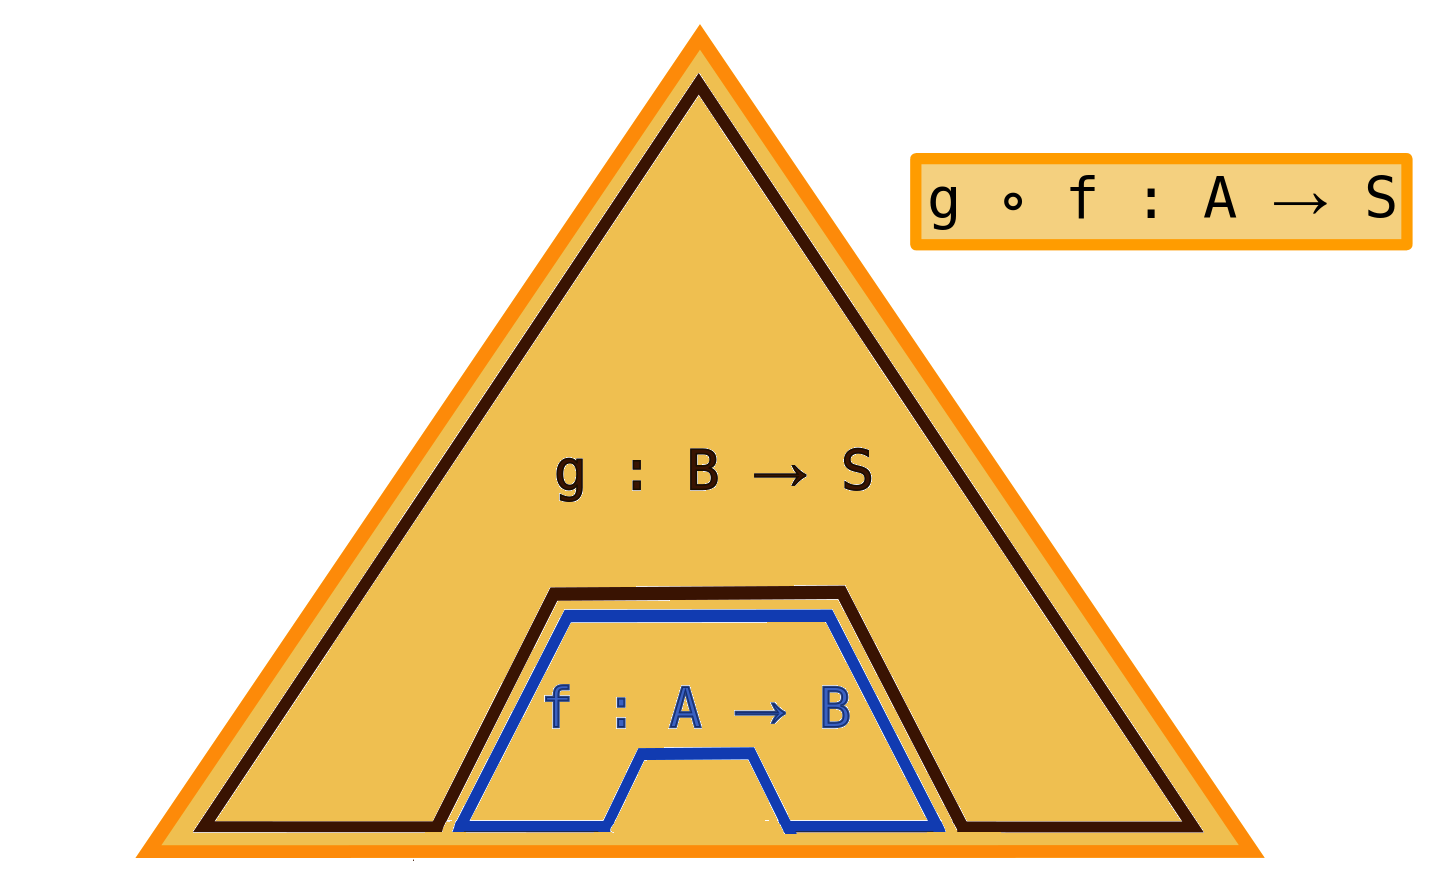
\includegraphics[width=0.45\textwidth]{img/contexts-dependence.png}
\caption{\todo{Make better graphics} Context for \t{A} in start
  category \t{S} depends on a context for \t{B}.}
\label{fig:context-dependence}
\end{figure}

Computing relevant contexts in a given start category \t{S} is done
once, in advance, for all possible hole types $H$ at the same time,
using fixpoint iteration. 
We model this in a top-down manner, where in the beginning, only the
start category \t{S} has a context, albeit a trivial one: ``do
nothing, you're already there!''. The other categories don't have a
context yet, but will get them during the process in the following
manner, referencing Figure~\ref{fig:context-dependence}. 

On the first round, we get to compute contexts for all categories
\t{B} that are arguments to some function \t{g : B $\rightarrow$ S}:
these contexts are simply the function \t{g} itself. On the second
round, we compute contexts for all categories \t{A} that are arguments
to some function \t{f~:~A~$\rightarrow$~B}; the context for such an
\t{A} is \t{g~$\circ$~f}. Each round unlocks more categories further
down from the start category, so we get to compute more contexts for
categories that depend on the newly unlocked ones, until all
categories have their contexts. Figure~\ref{fig:context-dependence}
shows the general pattern for categories \t{A} and \t{B} in start
category \t{S}.

The definition of contexts is mutually recursive, and can be seen as a
system of equations. The simple example with \t{f~:~A~$\rightarrow$~B}
and \t{g~:~B~$\rightarrow$~S} is expressed as follows.


\begin{EmptyItem}
\begin{array}{l @{\hspace{0.1cm}} l}
\textsf{contexts}(\t{S}) = & \{ \; id \; \} \\
\textsf{contexts}(\t{B}) = &  \{ \; C[g(\_)] \; | \; C \in
                             \textsf{contexts}(\t{S}) \} \\
\textsf{contexts}(\t{A}) = &  \{ \; C[f(\_)] \; | \; C \in
                             \textsf{contexts}(\t{B}) \} \\

\end{array}
\end{EmptyItem}


% \begin{table}[h]
% \ttfamily
% \begin{tabular}{p{0.1cm} l}
%      & \DataTypeTok{CtxS} \OtherTok{::=} \{ id \} \\
%    $\Bigg\{$  & \DataTypeTok{CtxB} \OtherTok{::=} \{ $f$ (\DataTypeTok{G} •) | $f$ $\leftarrow$ \DataTypeTok{CtxS} \}  \\
%      & \DataTypeTok{CtxA} \OtherTok{::=} \{ $f$ (\DataTypeTok{F} •) | $f$ $\leftarrow$ \DataTypeTok{CtxB} \} \\
% \end{tabular}
% \end{table}

\paragraph{Least solution} In the general case, these sets can be
infinite: think of functions of type \t{A~$\rightarrow$~A} and loops
of \t{A~$\rightarrow$~B} and \t{B~$\rightarrow$~A}. In such a case, we
want to find the {\em least} solution to such systems of equations.
The word \emph{least} means two separate things: (a) the fewest
trees that still use all the fields of the category, and (b) which are
of the smallest size (e.g. choosing \t{UttNP} over \t{PredAdj} for the
context of \t{NP}).

In contrast to the more intuitive bottom-up approach, top-down
computation is more efficient: we retrieve the fastest way to the
start category, because at each round, we consider contexts that we
already know to lead into the start category. We avoid functions
of type \t{B~$\rightarrow$~A} when computing the context for \t{B},
because we only consider functions whose goal type \emph{already has a
  context}; hence \t{g : B~$\rightarrow$~S} is the only candidate.



% To give an example, consider the context of \t{AP} in Spanish. \t{AdjCN : Adj
%   $\rightarrow$ CN $\rightarrow$ CN} would
% be a better local strategy than \t{PredAdj : NP $\rightarrow$ AP
%   $\rightarrow$ S}, because \t{AdjCN} lifts
% both singular and plural (masculine or feminine) forms of the \t{AP}
% into \t{CN} in one go, and
% \t{PredAdj} lifts only one form into an \t{S}. However, in order for
% the \t{CN} to make its way to \t{S}, four instances of \t{PredAdj}
% need to be called eventually, thus it is a better strategy to use
% \t{PredAdj} directly in the context of \t{AP}, because that results in
% the smallest trees: \emph{the blue house is big} vs. \emph{the house
%   is blue}.
% One way to compute that is to come up with a function $f$ such that if
% a set of contexts $X$ is a fixpoint of $f$, then $X$ is also a
% solution to the equations. We compute $X$ by fixpoint iteration.

%%%% EITHER this
% \input{chapters/gf-appendix.tex}

\paragraph{Algorithm}

% To compute relevant contexts with the start category \t{S} as a hole,
% we initialise the contexts as follows:


% \begin{EmptyItem}
% $\textsf{contexts}(S) = \{ \; id \; \}$ \\
% $\textsf{contexts}(H) = \{ \; \} \;\;\; : \; \forall H \neq S$
% \end{EmptyItem}

\noindent We express the set of relevant contexts for one hole type
$H$ in terms of the sets of relevant contexts for other hole types
$H'$, using the following definition:

\begin{EmptyItem}
$\textsf{contexts}(H) = \textsf{filter}(\;\{ C[F(\_)] \; | \; F \in H
\rightarrow H', \; C \in \textsf{contexts}(H') \}\;)$
\end{EmptyItem}

In words, to generate contexts with holes of type $H$, we enumerate
all functions $F$ that have a $H$ as an argument, and enumerate all
contexts $C$ that have the result type $H'$ of $F$ as a hole type, and
put $C$ and $F$ together to get a new context. Then, we apply a
function $\textsf{filter}$ to the result in order to filter out
redundant contexts, i.e. contexts whose uses of the strings of $H$ are
already covered by other contexts in the same set.

In order to compute all sets of contexts for all possible hole
categories $H$, we set up a system of equations. In general, this
system of equations is recursive, and we use a fixpoint iteration to
solve it, initialising the contexts as follows: $id$ for the start
category, and an empty set for all other categories. There is a guaranteed minimal solution, because the RHSs are monotonic
in $H'$. \todo{Kleene's fixed point theorem}

\begin{EmptyItem}
$\textsf{contexts}(S) = \{ \; id \; \}$ \\
$\textsf{contexts}(H) = \{ \; \} \;\;\; : \; \forall H \neq S$
\end{EmptyItem}
%  starting with $\textsf{contexts}(S) = \{ \; id \; \}$ for
% the start category, and $\textsf{contexts}(H)~=~\varnothing$ for
% each category $H$ that is not the start category.


It is important that we do not change the contexts for anything that
uses fewer or the same amount of fields. In the English example, it
would not serve any purpose to swap \t{PredAdj} for \t{AdjCN} in the
context of \t{AP}, because both choose the same (the only)
field. Furthermore, if we did that on an arbitrary basis, the sets
would not converge, and we wouldn't find a fixpoint.

However, the functions can be replaced in the case that we find a
function that covers strictly more fields than any of the previously found.
Assume that we added a whole new abstract syntax construction of type
\t{CN $\rightarrow$ NP}, which uses both singular and plural in one
sentence. Then we get just one context which covers two fields, and
thus we can throw away both \t{DetCN this} and \t{DetCN these} in
favour of the new construction.

So, the set of contexts for a category $H$ may change during the
fixpoint computation. It grows as we unlock contexts for more
categories, further down from the start category. It may also shrink,
if we find a single context that covers the fields from multiple,
previously computed, contexts. But most importantly, the list of
fields from $H$ that make it into the start category is growing
throughout the fixpoint computation. 



\subsection{Pruning the trees within one set of test cases} 

% \t{your} as definite,
% singular\footnote{In our grammar, \t{your} is singular just because we
%   decided---we could as well have made it plural, or include two
%   variants, \t{yourSg} and \t{yourPl}.} and non-contracting; \t{a} as
% indefinite, singular and non-contracting; \t{this} and \t{the} as
%  definite, singular and contracting; finally, \t{these} as definite,
%  plural and contracting. 

Sometimes we can further reduce test cases created for a single
function, taking advantage of the coercions in the grammar (explained
in Section~\ref{sec:PMCFG}).  Let us take as an example the function
\t{DetNP : Det $\rightarrow$ NP} for Dutch. As usual, the category
\t{Det} compiles into 8 concrete categories: combinations of singular
vs. plural, contracting vs.  non-contracting, and definite
vs. indefinite. But our grammar only has 5 determiners in total, out
of 8 possible combinations---does this mean that we cannot test
\t{DetNP} exhaustively with the small lexicon? Firstly, we look for
coercions of \emph{arguments} (\t{Det}) in the different concrete
versions of \t{DetNP}, and secondly, coercions of the \emph{goal
  category} (\t{NP}) used in the contexts.

\paragraph{Coercions of \t{Det} used by \t{DetNP}} Due to coercions, there are only 4
different type signatures for \t{DetNP}: definiteness is not relevant
when a \t{Det} is made directly into an \t{NP} (it only matters when
combining a determiner with an adjective). This brings us down to 4
arguments for \t{DetNP}, shown below.

\begin{itemize}
\setlength\itemsep{0em}
\item \t{DetNP : Det$_{*\text{,sg,noncontr}}$ $\rightarrow$ NP$_\text{sg,noncontr}$}
\item \t{DetNP : Det$_{*\text{,pl,noncontr}}$ $\rightarrow$ NP$_\text{pl,noncontr}$}
\item \t{DetNP : Det$_{*\text{,sg,contr}}$ $\rightarrow$ NP$_\text{sg,contr}$}
\item \t{DetNP : Det$_{*\text{,pl,contr}}$ $\rightarrow$ NP$_\text{pl,contr}$}
\end{itemize}

% \noindent Four looks better than eight, but we are missing a plural
% non-contracting determiner in the lexicon. However, we may still be
% able to test \t{DetNP} exhaustively---
\paragraph{Contexts for \t{NP}} The next step is to look at the \emph{contexts} for all goal
categories of \t{DetNP}, as shown in Table~\ref{tbl:nps}.  The
contracting \t{NP}s get two contexts, one to choose the full form and
other the contracted form.  The non-contracting ones only get one
context each, because their field for the contracted form is empty.


\begin{table}
\centering
%\resizebox{\textwidth}{!}{
\begin{tabular}{|l|l|l|l|} \hline
\t{NP$_\text{sg,noncontr}$} & \t{NP$_\text{pl,noncontr}$} & \t{NP$_\text{sg,contr}$}  & \t{NP$_\text{pl,contr}$}\\ \hline

\t{UttNP~\char`_}   & \t{UttNP~\char`_}   & \t{UttNP~\char`_} & \t{UttNP~\char`_} \\
 &  & \t{PredAdv \gray{any NP} (PrepNP on \char`_)} & \t{PredAdv
                                                      \gray{any NP} (PrepNP on \char`_)}
  \\ \hline
\end{tabular} %}
\caption{Contexts to showcase all strings of different concrete \t{NP}s in the Dutch grammar}
\label{tbl:nps}
\end{table}


\paragraph{Coercions of \t{NP} used in contexts} In addition, we look
for \emph{coercions} for all the goal categories. For instance, there
is one that covers all \t{NP}s; let us call that \t{NP$_*$}. This
tells us that there are functions that take \t{NP}, but don’t care
anything about about its parameters. One such example is \t{UttNP},
which just takes an \t{NP}, chooses the nominative form and makes it
into a standalone utterance.  There is another useful coercion, which
covers both singular and plural contracting \t{NP}s; we call that
\t{NP$_{*\text{,contr}}$}. It is used by \t{PrepNP}\footnote{Along
  with a similar coercion \t{NP$_{*\text{,noncontr}}$} for
  non-contracting \t{NP}s.}, which doesn't care about number, just
whether to merge its arguments or not.  In order to reduce the number
of test cases for any function \t{f~:~A~$\rightarrow$~B}, two
properties need to hold:
\begin{enumerate}
\item A number of concrete categories for \t{B} are interchangeable in a particular
context;
\item That context is one of those chosen to showcase \t{B}.
\end{enumerate}

\noindent With \t{NP$_*$} and \t{NP$_\text{*,contr}$}, both of these
properties hold.
%\t{UttNP : NP$_*$ $\rightarrow$ S}, and \t{PrepNP :
%  Prep  $\rightarrow$ NP$_\text{*,contr}$  $\rightarrow$ Adv}.
Thus, we only need to put one representative of \emph{any} \t{NP} into
the context \t{UttNP~\char`_}, and one representative of the
contracting \t{NP}s into the context \t{PredAdv~\gray{any NP}~(PrepNP~on~\char`_)}. 
The following trees would fit the description:

\begin{itemize}
\item[] \t{UttNP (DetNP this)}  \\
 \emph{deze} \\
 `this'
\item[] \t{PredAdv (DetCN a house) (PrepNP on (DetNP this)}  \\
\emph{een huis hierop} \\
`a house on this'
\end{itemize}


% Now, in order to compute a context for a coercion, we simply take
% the largest common subset of the categories that the coercion covers.
% The coercion \t{NP$_*$} is the most general, covering all \t{NP}s, so it only has the most general
% context: \t{UttNP~\char`_}, which is common to all non-coerced
% \t{NP}s. The other coercion \t{NP$_\text{*,contr}$} is more specific,
% so it has also a second context, only included for contracting
% \t{NP}s. Some contexts for coercions are shown in Table~\ref{tbl:npcs}.

% \begin{table}[h]
% \centering
% \begin{tabular}{|l|l|l|} \hline
% \t{NP$_*$}  &  \t{NP$_{*\text{,noncontr}}$} &\t{NP$_{*\text{,contr}}$}\\ \hline

% \t{UttNP~\char`_} & \t{UttNP~\char`_} & \t{UttNP~\char`_} \\
%                   & & \t{PredAdv \dots{} (PrepNP on \char`_)}
%   \\ \hline
% \end{tabular}
% \caption{Contexts to showcase all strings of some \t{NP}-coercions in the Dutch grammar}
% \label{tbl:npcs}
% \end{table}


\subsection{Pruning the trees to test the whole grammar}
\label{sec:pruning_all}

So far we have completely ignored that one tree can showcase more than
one function. In the Estonian example, we start
by testing \t{AdjCN} and end up with the following 8 trees, where
\t{PrepNP} is in the context: 
\t{PrepNP} \{ \stackanchor{\tt in}{\tt with} \}
             {\tt (DetCN} \{ \stackanchor{\tt this}{\tt these} \} 
             {\tt AdjCN}  \{\stackanchor{\tt blue}{\tt ready} \} 
             {\tt house)}.
In fact, these 8 trees cover all tests we would've needed for
\t{PrepNP} itself. Thus, it is possible to shrink the test cases
effectively, if one wants to test the whole grammar at one go.

\paragraph{Deterministic argument generation}
There is a simple way to detect redundancy in the generated trees. We
make the generation of arguments and contexts completely
deterministic, e.g. always choose the function that is alphabetically
first. Then, we would get a sentence such as ``the good house is
good'' for testing both \t{AdjCN} and \t{PredAdj}. The downside is
that the sentences can get boring to read, or even confusing, in the
style of ``the house gives the house the house''.

However, we can split the generation in two stages:
first stage is deterministic, where every noun is \t{house}, and we
can eliminate redundancies by just eliminating copies of the same
tree. Then, when we have a set of unique trees, we can substitute
individual words in them with other words in the same concrete
category.  A sentence such as ``the house gives the hill the
ham'' tests the same properties as the version with \emph{house} in every
role, but at least it is easier to keep track who does what, and
compare the translations of the same tree.

In practice, we only apply the first step, and let the sentences be
redundant. In Section~\ref{sec:evalGF}, we refer to total and unique
trees when generating tests for the whole grammar; ``unique trees''
means the number after removing duplicate trees that are generated to
test different functions, but happen to be the same.

\paragraph{Alternative priorities for context generation} The current
implementation of context generation prioritises minimal trees, such
as \t{UttNP} for \t{NP} instead of any other functions. As an alternative,
we could choose contexts where the \t{NP} can also use its
parameters, in addition to just showing all of its strings. Arguably,
it would tell more to the user to see a sentence like ``this house is
big'', formed with \t{PredAdj}, rather than just ``this house'',
formed by \t{UttNP}.

However, these alternative priorities are not implemented yet. With
the current scheme, we have found it a useful practice to hide
functions such as \t{UttNP}, which just lift a category into the start
category without introducing other arguments. For future, it would
make sense for a context to serve double purpose: show all of its
strings and (try to) use all of its parameters.
% Prefer contexts where there are no coercions

%\input{chapters/gf-additional-analyses.tex}

% \section{General algorithm}
% \label{sec:algorithm}

%  Here we present the algorithm for test suite generation. We refer
%  back to Section~\ref{sec:PMCFG} for the definition of \pmcfg{}.

% \input{chapters/gf-appendix.tex}



\section{Evaluation}
\label{sec:evalGF}

\begin{table}[h]
\centering
\resizebox{\textwidth}{!}{
\begin{tabular}{|lll|ll|ll|ll|ll|}
\hline
\multicolumn{3}{|r}{Concrete syntax $\rightarrow$}              &
                                                                   \multicolumn{2}{|c}{\bf Dutch} & \multicolumn{2}{|c}{\bf Spanish} & \multicolumn{2}{|c}{\bf Estonian} & \multicolumn{2}{|c|}{\bf Basque} \\
$\downarrow$ Grammar & \#funs+lex & \#trees  &
                                                          \#total & \#uniq & \#total & \#uniq & \#total & \#uniq  & \#total  & \#uniq \\ \hline
{\bf Noun phrases}     & \numOfFun{}+\numOfLex{}  
                               & \textgreater{}10,000  &    21    & 18     & 16     &15     & 33      & 27      & 40       & 36     \\ \hline
{\bf Phrasebook}       
                  & 130+160   & \textgreater{}480,000       
                                                       &   513    & 419     & 504     &382    & 610     & 505     & 538      & 503   \\ \hline
   {\bf Resource gr.}    & 217+446   & \textgreater{}500 billion  
                                                       &  21,370  & 19,825  & 19,689  & 16,662 & 13,733  & 9,194    & 100,967  & 64,390 \\ \hline
\end{tabular}}
\caption{Test cases for all functions in three grammars}
\label{results}
\end{table}


\begin{table}[h]

\centering
\begin{tabular}{|ll|l|l|l|l|}
\hline
\multicolumn{2}{|c|}{\bf Resource grammar function} & {\bf Dutch} & {\bf Spanish}
   & {\bf Estonian} & {\bf Basque} \\ \hline
 
\t{ComparA : A  $\rightarrow$ NP $\rightarrow$ AP~} & `stronger than you' & 10   & 4   & 20 & 6   \\
\t{RelNP~~~: NP $\rightarrow$ RS $\rightarrow$ NP~} & `a cat that I saw'  & 2    & 23 & 23 & 20   \\
\t{ComplVS : VS $\rightarrow$ S  $\rightarrow$ VP~} &`say that I sleep'  & 89   & 206 & 171 & 104 \\
\t{ReflVP~~: VPSlash $\rightarrow$ VP~~} & `see myself'        & 1034 & 890 & 343 & 1082 \\
\hline
\end{tabular}
\caption{Test cases for some individual functions in the resource
  grammar}
\label{results_indiv}
\end{table}

In order to evaluate our method, we generate test cases for grammars
of varying sizes, using the four languages presented earlier: Dutch, Spanish,
Estonian and Basque. These languages come from different language
families, and cover a wide range of grammatical complexity. Dutch and
Spanish are both Indo-European languages, with fairly simple nominal
morphology. Dutch features word order changes in subordinate and
question clauses, and separable prefixes in verb phrases (imagine
English behaving ``look something \emph{up} \~{} {\it up}looked''). 
Spanish has a large number of tenses and moods, and clitics for direct
and indirect objects, which attach to verbs.  To add some linguistic
variety, we include Estonian from the Finno-Ugric language family, and
Basque, an isolate language.  In contrast to Dutch and Spanish,
Estonian and Basque have a rich nominal morphology, with 14
grammatical cases in each. In addition, Basque has the most complex
verb morphology out of all the 4 languages, featuring agreement in
subject, object and indirect object.
The Dutch, Spanish and Estonian grammars behaved similarly to each other
and Basque significantly worse, both in execution time and examples
generated.

Table~\ref{results} shows the number of generated trees for 
in total for all syntactic functions in the three grammars, and
Table~\ref{results_indiv} shows some example functions from the resource grammar. 
As stated earlier, we do not consider generating test cases for all
functions an optimal way of testing a whole resource grammar from scratch;
this gives merely a baseline reduction from all possible trees up to a
reasonable depth. We introduce the grammars and comment on the results
in the following sections. 

\subsection{Grammars}

The first grammar is the toy example introduced earlier in this
article: \t{NounPhrases} with \numOfFun syntactic functions and
\numOfLex words in the lexicon. We wrote the concrete syntaxes from
scratch for each of the languages, instead of using the full resource
grammar and reducing it to only noun phrases. All four concrete
syntaxes were completed in less than an hour, by an experienced
grammarian with some knowledge in all the languages.

The second grammar is a mid-size application grammar: Phrasebook
\cite{ranta2010phrasebook}, with 42 categories such as \t{Person,
  Currency, Price} and \t{Nationality}, 160-word lexicon and 130
functions with arguments. As opposed to the trees that we have seen so far,
which only contain syntactic information, the trees in the Phrasebook
are much more semantic: for example, the abstract tree for the
sentence ``how far is the bar?'' in the Phrasebook is \t{PQuestion
  (HowFar (ThePlace Bar))}, in contrast to the resource grammar tree
{\tt \small UttQS (UseQCl (TTAnt TPres ASimul) PPos (QuestIComp
  (CompIAdv (AdvIAdv how\_IAdv (PositAdvAdj far\_A))) 
  (DetCN (DetQuant DefArt NumSg) (UseN bar\_N))))} for the same
sentence. Limiting up to depth 3, the Phrasebook grammar produces over
480,000 trees\footnote{Application grammars are usually
much more compact than resource grammars, hence depth 3 covers already
a lot of relevant trees.}.

%  All four concrete syntaxes were
% implemented using their respective resource grammars; thus if some
% Phrasebook function has a bug, say it produces ``Spaniard restaurant''
% instead of ``Spanish restaurant'', the problem could be in either grammar.
% In the first case, the resource grammar contains both \t{spanish\_A} ``Spanish'' and
% \t{spaniard\_N} ``Spaniard'', but the application grammarian has
% chosen the wrong function.
% In the second case, the application grammarian has correctly chosen
% \t{spanish\_A} from the resource grammar, but that word itself is
% linearised wrongly into ``Spaniard''.


The third grammar is a restricted version of the \gf{} resource grammar,
with 84 categories, 217 syntactic functions and 446 words in the
lexicon. Since all the languages did not have a complete
implementation, we simply took the subset of functions that was
common, and removed manually a couple of rare constructions and words
that are potentially distracting. 
This fragment produces hundreds of billions of trees already up to depth 5.
None of the resource grammars has been tested systematically before---for
the Estonian grammar \cite{listenmaa_kaljurand2014}, the morphological
paradigms were tested extensively against existing resources, but
syntactic functions were only tested with a treebank of 425 trees.

%: say, animate and inanimate nouns, ending in front vowel and back vowel.

\subsection{Execution time} We ran all the experiments on a MacBook Air
with 1,7 GHz processor and 8 GB RAM. For Phrasebook, it took just
seconds to generate the test suite for all languages. For the resource
grammar, Dutch and Estonian finished in 3--4 minutes. However, the
Basque resource grammar is noticeably more complex, and creating test
trees for all functions took almost three hours.

\subsection{Generated trees}

We report both total and unique trees: total trees are simply the sum
of all trees for all functions, and unique trees is the count after
removing duplicates, as explained in Section~\ref{sec:pruning_all}
(``the pizza gives the pizza the pizza'' style).

\paragraph{Grammar engineering vs. language typology}
As we can see in Table~\ref{results}, the number of trees differs between
languages. Table~\ref{results_indiv} shows some expected patterns in
individual functions. For instance, Basque and Estonian have more
complex noun morphology than Dutch, so \t{RelNP} needs more tests (20+
vs. 2): if the type for \t{NP} is a large inflection table, it needs
to be put in many contexts. However, if the question was purely about
language complexity, we would expect Spanish to behave more like
Dutch: both have only 2 cases, nominative and accusative. 
%  Looking at the implementation of \t{NP} in the Spanish grammar, we
% discover that it includes 14 fields.

In fact, around 80 \% of the code in the Spanish grammar is inherited
from a common module to all Romance languages; thus the implementation
is meant to be as general as possible, and support all distinctions
that appear in some language, not necessarily in Spanish itself. In
this case, the pan-Romance category for \t{NP} includes nominative,
accusative, dative and genitive as cases in the inflection table, even
though the latter two are realised as just prepositions (\emph{a} and
\t{de}) in Spanish. In addition, all cases include a stressed and
unstressed form---this makes for 8 fields in total.

% In addition to nominative and accusative, which differ for
% personal pronouns (\emph{yo} `I' vs. \emph{m\'{i}} `me'), a few
% prepositions are also encoded as cases, perhaps to generalise among
% all Romance languages so that they can share code. In addition,
% each ``case'' includes a stressed and unstressed form

As another example, Basque, Spanish and Dutch have more complex verb
phrases (for different reasons!) than Estonian, so they need more test
cases to test \t{ReflVP}. This time it is not only about the contexts,
but also the arguments: \t{ReflVP} takes a \t{VPSlash}, which has many
parameters, so the tool needs to create many examples to cover all
different concrete categories for \t{VPSlash}.

In general, we believe the number of test cases has both language
typological and grammar engineering reasons. Other resource
grammarians have reported significant differences in complexity
between implementations: \citet{enache2010} report a
200-time reduction in the number of concrete rules after changing the
implementation of clitics in verb phrases.

To further explore the effect of grammar engineering vs. inherent
language complexity, it would be interesting to generate test cases
for two different implementations of the same language.  However,
there is not much material to explore---writing a full resource
grammar is several months' effort, thus writing a second
implementation for a language that already is in the RGL is hardly a
justifiable use of resources. We could explore related languages, but in
practice they are often based on one another, either by copying an
existing one and modifying it (e.g. Afrikaans based on Dutch, Estonian
on Finnish), or writing a parameterised module from the beginning,
with the intention of fitting several languages (e.g. Romance and
Scandinavian languages). 

% If there was an easy way to convert other grammar formalisms into
% \pmcfg{} (or more specifically, into the particular format that our
% tool reads \cite{angelov2010pgf}), 
% get a resource
% grammar written in some different formalism, convert it to a \pmcfg{}, and then compare the generated test cases.

\paragraph{Two different implementations of Basque noun phrase grammar}

Given the lack of large-scale language resources with different
implementations, we experimented with the noun phrase grammar for
Basque. In the first implementation, the one described earlier in this
chapter, we implemented nominal morphology using inflection tables,
and syntactic functions choose the correct case for each purpose. In
another grammar, we used the Basque resource grammar, which has
implemented nouns as stems, and syntactic functions concatenate
suffixes to the stems.  In the stem-based grammar, nouns have
phonological features as inherent parameters, in order to attach the
correct form of the inflectional morphemes. For test case generation,
this had the added benefit or curse of implicitly testing morphology
as well. For instance, \t{AdjCN} needs to generate test cases with the
arguments \{\stackanchor{\tt \small good}{\tt \small small}\} {\tt
  house}, just because \emph{good} ends in a consonant and
\emph{small} in a vowel. 
%Usually, this level of detail is not encoded in the \gf{} grammar.

\begin{table}[h]

\centering
\begin{tabular}{| p{2.3cm} | l | l |}
\hline
{\bf Function} & {\bf Inflection table}
   & {\bf Stems} \\ \hline
 
\t{PredAdj}, \t{PredAdv}, \t{UttNP}, \t{PrepNP}  & 1, 1, 1, 1 & 1, 1,
                                                                1, 1
  \\ \hline
\t{DetNP}    & 3 & 4   \\ \hline
\t{DetCN}    & 3 & 4   \\ \hline
\t{AdjCN}    & 7 & 4   \\ \hline
\t{AdvCN}    & 7 & 4   \\ \hline
% \t{UttNP}    & 1 & 1  \\
% \t{PredAdj}  & 1 & 1  \\
% \t{PredAdv}  & 1 & 1    \\
% \t{DetNP}    & 3 & 4   \\
% \t{DetCN}    & 3 & 4   \\
% \t{PrepNP}   & 1 & 1   \\
% \t{AdjCN}    & 7 & 4   \\
% \t{AdvCN}    & 7 & 4   \\ \hline
{\bf Total:} & {\bf 24} & {\bf 20} \\ 
\hline
\end{tabular}
\caption{Two versions of Basque concrete syntax for noun phrase grammar}
\label{basque_versions}
\end{table}

In the version based on inflection tables, \t{AdjCN} needs only one
adjective and one noun to form the test cases, for instance \t{AdjCN
  small house}.
This tree is then put in 7 different contexts, in order to showcase
all the different fields in the \t{CN}.

\begin{EmptyItem}
\begin{Highlighting}[]
UttNP (DetCN a _)
UttNP (DetCN your _)
UttNP (DetCN the _)
PredAdv \gray{any NP} (PrepNP on (DetCN your _))
PredAdv \gray{any NP} (PrepNP from (DetCN your _))
PredAdv \gray{any NP} (PrepNP on (DetCN the _))
PredAdv \gray{any NP} (PrepNP from (DetCN the _))
\end{Highlighting}
\end{EmptyItem}

\noindent In Section~\ref{gf-testing-examples}, we described the
placement of determiners in Basque. In the hand-written fragment for
noun phrases, we introduced a parameter in the \t{Det} type, which
controls the placement of the determiner, and which form it chooses
from the \t{NP}. We can see quite clearly which part comes from where:
\t{AdjCN} only creates an inflection table, and the rest of the
context chooses different forms.


In contrast, the stem-based grammar creates much more unwieldy
arguments for \t{AdjCN}. We explained the choice of good and small
already, due to phonetic features as inherent parameters, but the full
trees are more complex, as in the following: 

\begin{EmptyItem}
\t{AdjCN \{\stackanchor{\tt \small
    good}{\tt \small small}\} (AdvCN (PrepNP without (DetCN a house))
  house)} \\ `good/small house without a house'.
\end{EmptyItem}

This is because in the full resource grammar, there is no parameter
for the modifier and determiner placement, instead, each \t{CN} just
includes fields for heavy and non-heavy modifier, and all determiners
include the fields for pre- and postdeterminer. This way the functions
don't need to include any pattern matching, just concatenate
\t{det.pre ++ cn.heavyMod ++ cn.noun ++ cn.lightMod ++ det.post}, and
any of these fields may be empty. The downside is that, in order to
generate a minimal number of test cases, the best strategy is to
generate a test case where the fewest possible of these strings are
empty. This leads into fewer examples, but they are harder to read.

The number of generated test cases doesn't differ much in this
example. Furthermore, the version implemented with resource grammar
includes many unnecessary distinctions for such a small grammar: for
instance, each of the two trees generated for \t{AdjCN} are put in
singular and plural contexts, which is completely irrelevant in the
scope of our tiny grammar.  Thus we cannot draw any conclusions which
strategy leads to more test cases. However, just reading the generated
44 (20+24) trees suggests that the full resource grammar generates less
readable test cases.

% For
% instance, each of the two trees generated for \t{AdjCN} are put in two
% contexts each: singular and plural. Strictly speaking, even singular
% and plural are unnecessary for this particular grammar, but the Basque
% resource grammar includes a variable number in \t{CN}, because in the
% full resource grammar, \t{CN} may be modified by a relative clause,
% which has to keep its agreement open.




% Why the RG version didn't include \t{your}: because all determiners
% have two fields in the RG, \t{pre} and \t{post}, and no matter if one
% is empty, all applications of \t{DetCN} are just implemented as
% \t{det.pre ++ noun ++ det.post}. So there is no parameter in the RG
% for ``det comes before/det comes after''.

\subsection{Qualitative analysis} 

The Basque resource grammar is still a work in progress, and the test
sentences showed serious problems in morphology. We thought it
premature to get a fluent speaker to evaluate the grammar, because the
errors in morphology would probably make it difficult to assess syntax
separately. Phrasebook was implemented using the resource grammar, so
it was equally error-ridden.

For Estonian, we read through all the Phrasebook test sentences. These
505 sentences showed a handful of bugs---all coming from Phrasebook
itself, not from the resource grammar. Most were individual words
having the wrong inflection paradigm (the right one exists in the
resource grammar, but wrong one was chosen by the application
grammarian), but there were also some bugs in more general
functions: for example, using a wrong form of nationality when applied
to a human and when to an institution, along the lines of ``Spaniard
restaurant''. As expected, Phrasebook sentences were easier to read,
and made more sense semantically than sentences from the resource
grammar.

We have been developing the tool by testing it on the Dutch resource
grammar---this process is described in more detail in
Section~\ref{dutch-experiment}. During 6 months, we have committed 22
bugfixes on Dutch in the \gf{} main repository. (In the name of
honesty, a few of the bugs were caused by our earlier “fixes”—that was
before we had implemented the comparison against an older version of
the grammar.) One of the bugs found in Dutch was also present in other
languages, so we fixed it in German and English.

\section{Fixing the Dutch grammar}
\label{dutch-experiment}

In this section, we describe the long-term project of fixing bugs in
the Dutch resource grammar. The reader uninterested in details of
grammar writing may well skip the section and go to conclusions.


\subsection{Experimental setup}\label{experimental-setup}

We describe a collaboration between a grammarian (the author), who is an
expert in \gf, and a native Dutch speaker. We wanted to investigate the
feasibility of this division of labour: ideally, the tester can be any
native speaker, with no skills in \gf{} whatsoever. In our case, the tester
also had \gf{} skills, but did not have access to the grammar, only to the
produced sentences.

We generated a set of test sentences for each function in Dutch, with
English translations, and gave them to the native tester to read. The
tester replied with a list of sentences that were wrong, along with
suggestions for improvement. Communication between the grammarian and
the tester was conducted via email.

\subsection{Types of bugs}\label{types-of-bugs}

We can classify the bugs in two dimensions: how easy it is to understand
what the problem is, and how easy it is to fix the grammar. Ease of
understanding is relative to the grammarian: a trained linguist who is
fluent in Dutch would have easy time pinpointing the error from the
generated test cases, having both intuition and technical names for
things. Ease of fixing is relative to the grammar: a given grammatical
phenomenon can be implemented in a variety of ways, some of which are
harder to understand. Say that relative clauses are implemented as
terrible spaghetti code in a Dutch grammar, but very elegantly in a
German grammar, and both have a bug that results in a similar
ungrammatical sentences. In such a case, the problem would be equally
easy to understand in both languages, but fixing the bug would be easier
in the German grammar.

In more concrete terms, \emph{easy to fix} means just some local changes
in a single function. In contrast, bugs that are \emph{hard to fix}
usually involve modifying several functions, restructuring the code or
adding new parameters.

\subsubsection{Easy to understand, easy to
fix}\label{easy-to-understand-easy-to-fix}

Perhaps the easiest bug to fix is to correct a wrong lexical choice.
Below is an example feedback from the tester.

\begin{quote}
``opschakelen'' is not the right translation of ``switch on''.
``aanzetten'' or ``aandoen'' is better.
\end{quote}

Other examples include wrong inflection or agreement, e.g.~the polite
second person pronoun should take the third person singular verb form,
but was mistakenly taking second person forms.

Typically, bugs that are due to an almost complete implementation are
easy to fix. For instance, particle verbs were missing the particle in
future tense. Looking at the generated sentences, we could see the
particle being in the right place in all other tenses, except for the
future. There was a single function that constructed all the tenses, and
looking at the source code, we could see the line
\texttt{++ verb.particle} in all other tenses except the future. In such
a case, fixing the bug is fairly trivial.

\subsubsection{Easy to understand, hard to
fix}\label{easy-to-understand-hard-to-fix}
Dutch negation uses two strategies: the clausal negation particle
\emph{niet} `not', and the noun phrase negation \emph{geen} `no'. There
are some subtleties in their usage---the following quote comes from the
tester:

\begin{quote}
In any case, one can never say ``eet niet wormen'' (don't eat worms,
literally).\\That should always be ``eet geen wormen'' (don't eat worms,
correctly translated)
\end{quote}

\noindent We sent three more sentences as follow-up, and got the
following answer:

\begin{quote}
eet niet deze wormen - maybe OK?, feels strange\\eet deze wormen niet -
definitely OK\\eet niet 5 wormen - definitely OK
\end{quote}

\noindent From the feedback, it was fairly easy to see the pattern:
clauses with indefinite noun phrases (\emph{a} worm, \emph{worms}) use
noun phrase negation, but if the noun phrase has any other determiner
(\emph{these} worms, \emph{five} worms), then clausal negation is
appropriate. 

In the grammar, this fix required changes to 13 categories. Not all
categories had to be changed manually, but e.g.~a change in \texttt{NP}
changes all categories that depend on it, such as \texttt{Comp} and
\texttt{VP}. Depending on how modularly the grammar is implemented, this
means that some functions that operate on \texttt{VP} or \texttt{Comp}
need to be changed too, when \texttt{NP} changes.

\subsubsection{Hard to understand, easy to fix}\label{hard-to-understand-easy-to-fix}

The following two sentences were generated by the same function, which
turns superlative adjectives and ordinal numbers into complements. The
tester reported problems with both of them, as follows:

\begin{quote}
ik wil roodst worden --\textgreater{} ik wil \textbf{het} roodst worden
(`I want to become reddest')\\ik wil \sout{tiend} worden
--\textgreater{} ik wil \textbf{tiende} worden (`I want to become
tenth')
\end{quote}

\noindent We gave some more sentences to the tester, and got the following
feedback:

\begin{quote}
ik wil linker worden --\textgreater{} ik wil \textbf{de} linker worden
(`I want to become left')\\ik wil 224e worden = OK (`I want to become
224th')
\end{quote}

This small example gave at least three different ways of using these
complements: for numerals, no article and -e at the end (\emph{tiende}
`tenth'); for superlative adjectives, the article \emph{het} and no -e
at the end of the adjective (\emph{het roodst} `the reddest'), and for
a class of adjectives like \emph{left} and \emph{right}, the article
\emph{de} (\emph{de linker} `the left one').

In addition, the grammar has a separate construction for combining a
numeral and a superlative adjective, e.g. ``tenth best''. Since the
tests were generated per function, the main tester didn't read those
sentences at the same time. After noticing the additional function, we
asked another informant how to say \emph{Nth best}, and got an
alternative construction \mbox{\emph{op~(N-1)~na~best}}. Eventually, we got an
answer that the strategy used for superlative adjectives, i.e.~with the
article \emph{het} and no -e in the number, is acceptable.

Once it was clear to the grammarian how to proceed, fixing the bug was
easy. There was already a parameter for the adjective form: attributive
in two forms (strong and weak) and one predicative, and the different
classes of adjectives corresponded to the abstract syntax of the \gf{}
Resource Grammar Library (RGL).
Thus it was easy to modify the predicative form in a different way for
different adjective types. Earlier, the predicative was just identical
to the other attributive form, but now the \texttt{AP} type actually
contains 3 different strings for superlatives: \emph{beste} and
\emph{best} for attributive and \emph{het best} for predicative.
Adjectives in positive or comparative don't get the article: \emph{good}
is just \emph{goede}, \emph{goed} and \emph{goed} (not \emph{*het
goed}).

If there hadn't been already a parameter for different adjective forms,
or if the classes of words with different behaviours hadn't corresponded
to the RGL categories, then this bug would have required more work to fix.

\subsubsection{Hard to understand, hard to
fix}\label{hard-to-understand-hard-to-fix}

As an example of a problem that was hard to understand and hard to fix,
we take the agreement of a reflexive construction in conjunction with a
verbal complement. More concretely, consider the following sentences:

\begin{itemize}
\itemsep1pt\parskip0pt\parsep0pt
\item
  I like myself / you like yourself / \ldots{}
\item
  I help [ you like yourself / them like themselves / \ldots{} ]
\end{itemize}

These seem like reasonable choices: if the object of liking was \emph{I}
in the second example, the pronoun wouldn't be \emph{myself} but \emph{me}: ``I
help you like me''.
In the \gf{} grammar, these sentences are constructed in a series of steps:
\newpage
\begin{EmptyItem}
\begin{Highlighting}[]
\DataTypeTok{PredVP} \NormalTok{(}\DataTypeTok{UsePron} \NormalTok{i_Pron)}
       \NormalTok{(}\DataTypeTok{ComplSlash}
           \NormalTok{(}\DataTypeTok{SlashV2V} \NormalTok{help_V2V}
               \NormalTok{(}\DataTypeTok{ReflVP}
                 \NormalTok{(}\DataTypeTok{SlashV2a} \NormalTok{like_V2)}
               \NormalTok{)}
           \NormalTok{)}
           \NormalTok{(}\DataTypeTok{UsePron} \NormalTok{they_Pron)}
       \NormalTok{)}
\end{Highlighting}
\end{EmptyItem}

The innermost subtree is \texttt{SlashV2a like\_V2}: the transitive verb
\emph{like} is converted into a \texttt{VPSlash} (i.e.
\texttt{VP\textbackslash{}NP}). Right after, the function
\texttt{ReflVP} fills the \texttt{NP} slot and creates a \texttt{VP}.
However, no concrete string for the object is yet chosen, because the
reflexive object depends on the subject. The status of the VP is as
follows at the stage \texttt{ReflVP (SlashV2a like\_V2)}:

\begin{EmptyItem}
\begin{Highlighting}[]
    \NormalTok{s }\FunctionTok{=} \StringTok{"like"} \NormalTok{;}
\NormalTok{ncomp }\FunctionTok{=} \NormalTok{table \{ }\DataTypeTok{I} \OtherTok{=>} \StringTok{"myself"} \NormalTok{; }\DataTypeTok{You} \OtherTok{=>} \StringTok{"yourself"} \NormalTok{; … \} ;}
\NormalTok{vcomp }\FunctionTok{=} \NormalTok{[] ;}
\end{Highlighting}
\end{EmptyItem}

If we added a subject at that point, the subject would choose the
appropriate agreement: \emph{I} like \emph{myself}, \emph{you} like
\emph{yourself}. But instead, we add another slash-making construction,
\texttt{SlashV2V help\_V2V}. Now the new verb \texttt{help\_V2V}, which
takes both a direct object and a verbal complement, becomes the main
verb. The old verb \emph{like} becomes a verbal complement.

\begin{EmptyItem}
\begin{Highlighting}[]
    \NormalTok{s }\FunctionTok{=} \StringTok{"help"} \NormalTok{;}
\NormalTok{ncomp }\FunctionTok{=} \NormalTok{table \{ }\DataTypeTok{I} \OtherTok{=>} \StringTok{"myself"} \NormalTok{; }\DataTypeTok{You} \OtherTok{=>} \StringTok{"yourself"}\NormalTok{; … \} ;}
\NormalTok{vcomp }\FunctionTok{=} \StringTok{"like"} \NormalTok{;}
\end{Highlighting}
\end{EmptyItem}

The next stage is to add an \texttt{NP} complement \texttt{they\_Pron},
using the function \texttt{ComplSlash}. The standard way for
\texttt{ComplSlash} is to insert its \texttt{NP} argument into the
\texttt{ncomp} table, taking the \texttt{vcomp} field along.

In the old buggy version, \texttt{ComplSlash} just concatenated the new
object and the \texttt{vcomp} with the reflexive that was already in the
\texttt{ncomp} table. But the scope of the reflexive was wrong: when
adding an object to a \texttt{VPSlash} that has a verbal complement
clause, the object should complete the verbal complement and pick the
agreement. It is not in the scope for the subject.\\
The old behaviour was as follows:

\begin{EmptyItem}
\begin{Highlighting}[]
    \NormalTok{s }\FunctionTok{=} \StringTok{"help"} \NormalTok{;}
\NormalTok{ncomp }\FunctionTok{=} \NormalTok{table \{ }\DataTypeTok{I} \OtherTok{=>} \AlertTok{"them like myself"} \NormalTok{; }\DataTypeTok{You} \OtherTok{=>} \AlertTok{"them like yourself"}\NormalTok{; … \} ; }
\NormalTok{vcomp }\FunctionTok{=} \NormalTok{[] ;}
\end{Highlighting}
\end{EmptyItem}

After fixing the bug, the table was as follows:

\begin{EmptyItem}
\begin{Highlighting}[]
    \NormalTok{s }\FunctionTok{=} \StringTok{"help"} \NormalTok{;}
\NormalTok{ncomp }\FunctionTok{=} \NormalTok{table \{ _ }\OtherTok{=>} \StringTok{"them like themselves"} \NormalTok{\} ;}
\NormalTok{vcomp }\FunctionTok{=} \NormalTok{[] ;}
\end{Highlighting}
\end{EmptyItem}

But this turned out not to be a perfect solution. The exception to this
is when the \texttt{VPSlash} is formed by
\texttt{VPSlashPrep : VP -\textgreater{} Prep -\textgreater{} VPSlash}.
With the changes to \texttt{ComplSlash}, we suddenly got sentences such
as ``{[}I like \emph{ourselves}{]} without \emph{us}''. This would be a
valid linearisation for a tree where {[}\emph{ourselves} without
\emph{us}{]} is a constituent (such a tree is formed by another set of
functions and was linearised correctly), but in this case, the order of
the constructors is as follows:

\begin{itemize}
\item
  \t{ReflVP like}

\begin{EmptyItem}
\begin{Highlighting}[]
    \NormalTok{s }\FunctionTok{=} \StringTok{"like"} \NormalTok{;}
\NormalTok{ncomp }\FunctionTok{=} \NormalTok{table \{ }\DataTypeTok{I} \OtherTok{=>} \StringTok{"myself"} \NormalTok{; }\DataTypeTok{You} \OtherTok{=>} \StringTok{"yourself"} \NormalTok{; … \} ;}
\end{Highlighting}
\end{EmptyItem}

\item
  \t{VPSlashPrep (ReflVP like) without}

\begin{EmptyItem}
\begin{Highlighting}[]
    \NormalTok{s }\FunctionTok{=} \StringTok{"like"} \NormalTok{;}
\NormalTok{ncomp }\FunctionTok{=} \NormalTok{table \{ }\DataTypeTok{I} \OtherTok{=>} \StringTok{"myself"} \NormalTok{; }\DataTypeTok{You} \OtherTok{=>} \StringTok{"yourself"} \NormalTok{; … \} ;}
 \NormalTok{prep }\FunctionTok{=} \StringTok{"without"}
\end{Highlighting}
\end{EmptyItem}

\item \t{ComplSlash (VPSlashPrep (ReflVP like) without) we\_Pron)}

\begin{EmptyItem}
\begin{Highlighting}[]
    \NormalTok{s }\FunctionTok{=} \StringTok{"like"} \NormalTok{;}
\NormalTok{ncomp }\FunctionTok{=} \NormalTok{table \{ }\DataTypeTok{I} \OtherTok{=>} \StringTok{"myself"} \NormalTok{; }\DataTypeTok{You} \OtherTok{=>} \StringTok{"yourself"} \NormalTok{; … \} ;}
  \NormalTok{adv }\FunctionTok{=} \StringTok{"without us"}
\end{Highlighting}
\end{EmptyItem}

\end{itemize}

The desired behaviour is to put the complement into an adverbial slot
and keeping the agreement in \texttt{ncomp} open to wait for the
subject. But the following happened after our initial changes in
\texttt{ComplSlash}:

\begin{EmptyItem}
\begin{Highlighting}[]
    \NormalTok{s }\FunctionTok{=} \StringTok{"like"} \NormalTok{;}
\NormalTok{ncomp }\FunctionTok{=} \NormalTok{table \{ _ }\OtherTok{=>} \AlertTok{"ourselves without us"} \NormalTok{\} ; }
\end{Highlighting}
\end{EmptyItem}

To fix this problem, we added another parameter to the category
\texttt{VPSlash}. All \texttt{VPSlash}es constructed by
\texttt{VPSlashPrep} have now a \texttt{missingAdv} set True: this tells
that the \texttt{VPSlash} is not missing a core argument, so it
shouldn't affect the agreement. With the new parameter,
\texttt{ComplSlash} can now distinguish when to choose the agreement
from the \texttt{NP} argument and when to leave it open for the subject.

All in all, this was a complex phenomenon, and there were different
interpretations in the RGL. For the Scandinavian languages, the
behaviour was as we expected, but for English and German, it was
similar to Dutch. We fixed the grammar for all three languages (Dutch,
English and German), using the same strategy.

\subsection{Numbers}\label{numbers}

How many bugs were fixed and how many were of which kind? We skip the
ease of understanding, and just classify the bugs by how easy they were to fix.

\subsubsection{Easy to fix:}\label{easy-to-fix}

\begin{enumerate}
\def\labelenumi{\arabic{enumi}.}
\itemsep1pt\parskip0pt\parsep0pt
\item
  Several lexical changes.
\item
  Several inflection fixes.
\item
  \t{youPol\_Pron} had agreement of \t{Sg P2}, changed it to \t{Sg P3} so that a
  correct reflexive pronoun is chosen.
\item
  Choose always stressed forms of personal pronouns.
\item
  Change agreement in conjunctions
\item
  Extra prefix in prefix verbs for perfect tense
\item
  Missing participle in future tense
\item
  Plural imperatives
\item
  Two bugs in postmodifier \texttt{AP}s: placement and the adjective
  form. ``een getrouwde worm'' is correct, but a heavier \texttt{AP}
  should become a postmodifier, and in that case, the adjective form
  should be without the e at the end.
\item
  Superlatives and ordinals
\item \t{DetQuant} (and \t{DetQuantOrd}) combining a \t{Quant} and a
  \t{Num}, and when \t{Num} is an actual digit, both \t{Quant} and the \t{Num}
  contribute with a string, thus becoming \emph{een 1 huis} `a 1
  house'.
\end{enumerate}

\subsubsection{Hard to fix}\label{hard-to-fix}

\begin{enumerate}
\def\labelenumi{\arabic{enumi}.}
\itemsep1pt\parskip0pt\parsep0pt
\item
  Add missing inflected forms for past participles + add missing
  linearisation for the function \texttt{PastPartAP}
\item
  Preposition contraction
\item
  Negation patterns (\emph{niet} and \emph{geen})
\item
  Variety of word order weirdness in verbal complements: affected
  several functions, fixed in several functions
\item
  Scope of \texttt{ReflVP} with \texttt{VPSlash}
\end{enumerate}

\subsubsection{Time spent by testers + how many sentences they
read}\label{time-spent-by-testers-how-many-sentences-they-read}

Tester 1 has read probably hundreds or thousands of sentences by now.
 \todo{get some more accurate numbers}

Tester 2 has been used as a backup when Tester 1 was not available and the
grammarian wanted quick feedback. She's read roughly tens of sentences.

\section{Conclusion and future work}
\label{gf-future}

We have presented method for automatically generating minimal and
exhaustive sets of test cases for testing grammars.  We have found the
tool useful in large-scale grammar writing, in a context where
grammars need to be \emph{reliable}.

One problem we have encountered is that the test sentences from
resource grammars are often nonsensical semantically, and hence a
native speaker might intuitively say that a sentence is wrong, even
though it is just unnatural.  For instance, the function \t{AdvQVP}
covers constructions such as ``you did \emph{what}?''. However, the
function itself is completely general and can take any verb phrase and
any question adverb, thus bizarre combinations like ``you saw the dog
why'' may appear in the generated test cases. If the grammar is purely
syntactic, we would need external tools to ensure semantic coherence,
but if the grammatical categories already include semantic
distinctions, e.g. limiting the subject and indirect object of
\emph{give} into humans, that naturally restricts the generated test
suite.


So far the only mode of operation is generating test cases for a
single function. 
% Generating test cases to all trees often leads to redundant
% trees---as we noted in Section~\ref{sec:wishlist_comments}, the trees
% that are needed to test \t{AdjCN} in Estonian are exactly the same
% trees we need to test \t{PrepNP}, even though the functions are
% seemingly separate. 
As future work, we are planning to add a separate
mode for testing the whole grammar from scratch: intentionally create
trees that test several functions at once.
We have an implementation only for \gf{} grammars so far, but the
general method works for any grammar formalism that can be compiled
into \pmcfg{}. \gf{} already supports reading context-free grammars,
so testing any existing \cfg{} is a matter of some preprocessing. 

